
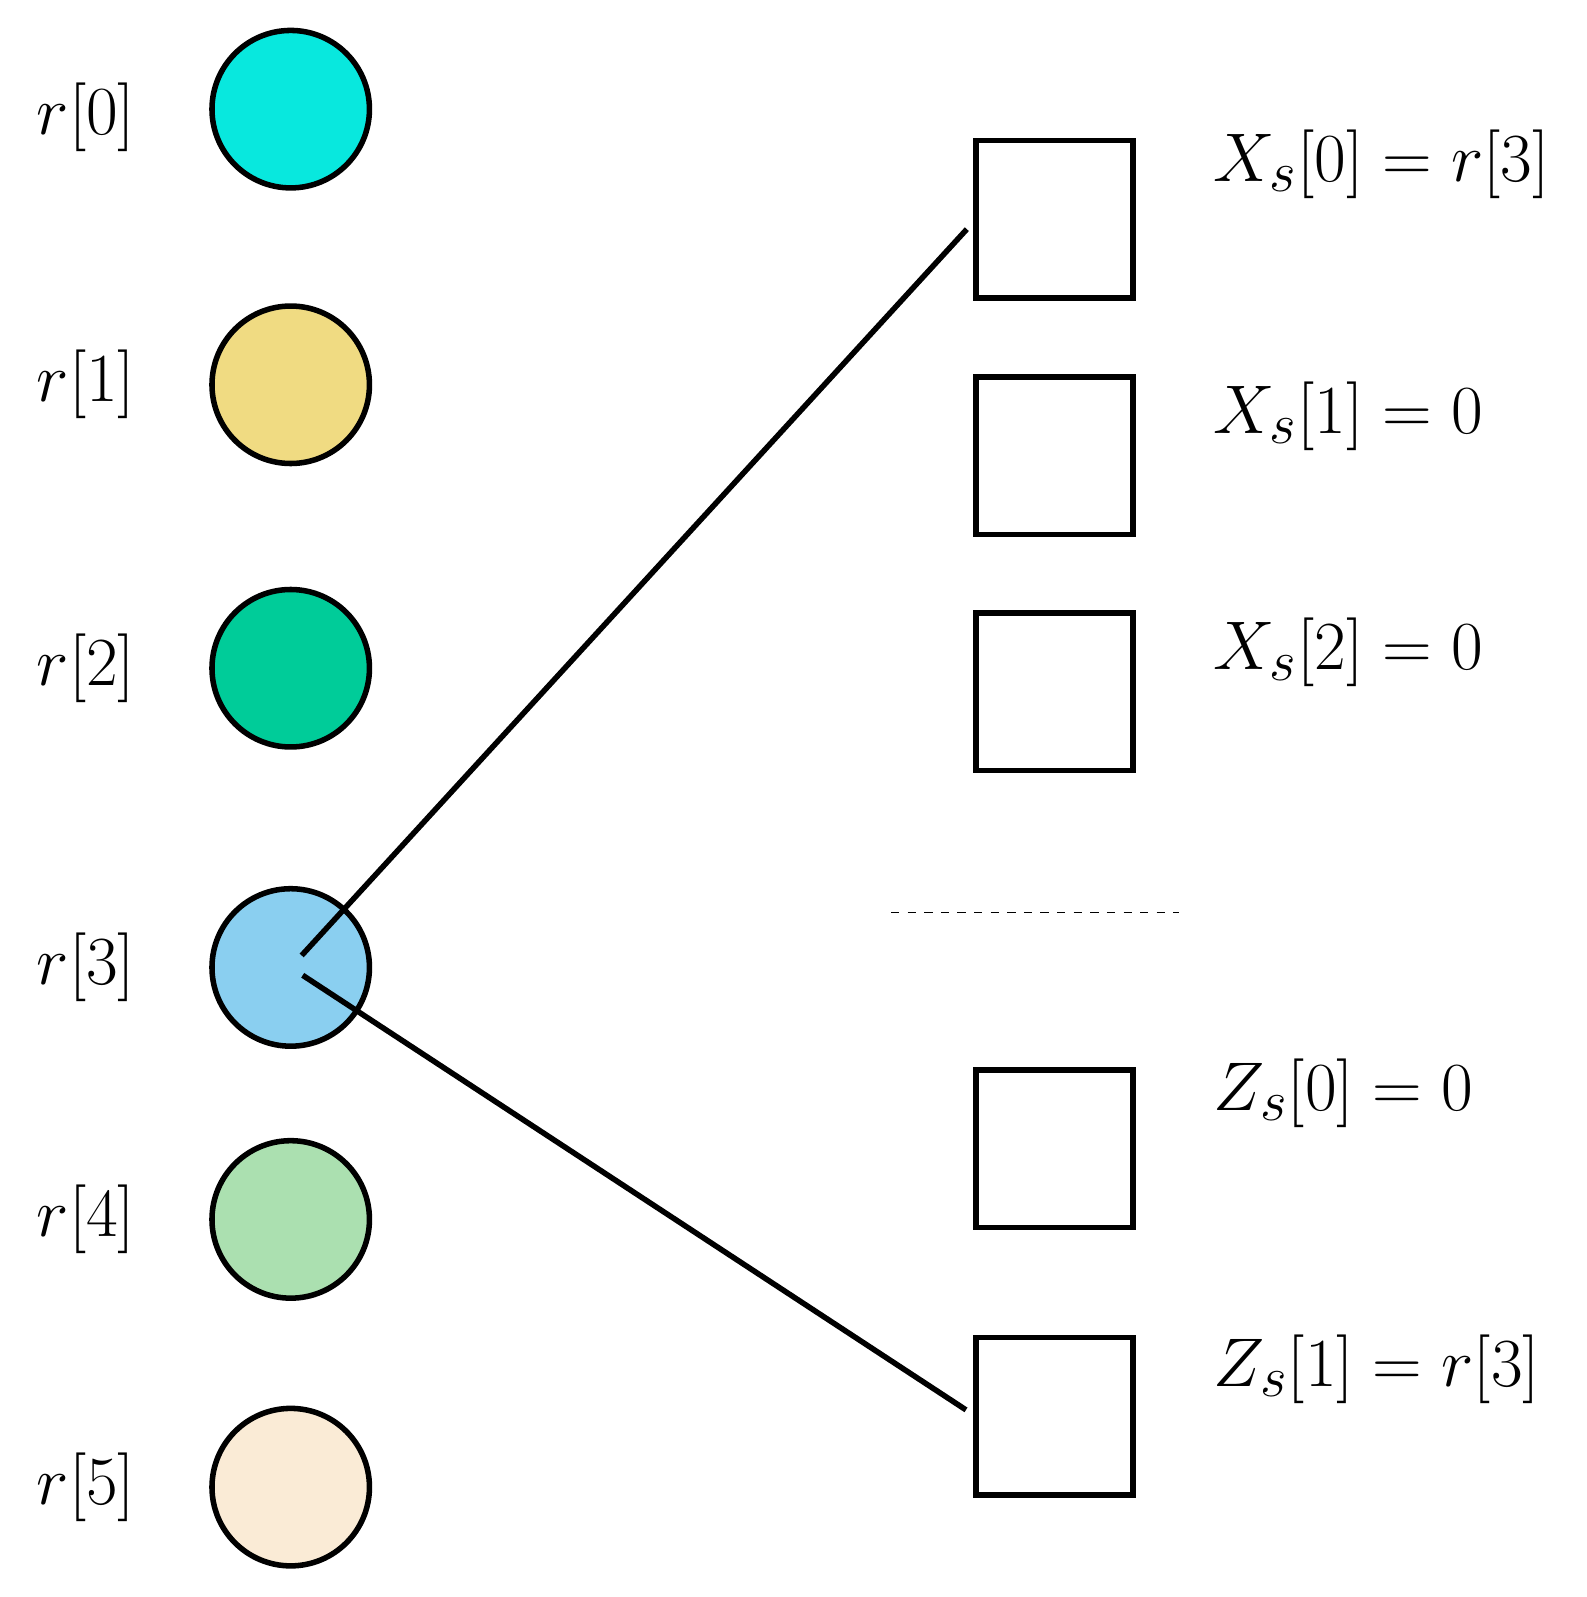
\begin{tikzpicture}

\definecolor{brightturquoise}{rgb}{0.03, 0.91, 0.87}
\definecolor{buff}{rgb}{0.94, 0.86, 0.51}
\definecolor{caribbeangreen}{rgb}{0.0, 0.8, 0.6}
\definecolor{celadon}{rgb}{0.67, 0.88, 0.69}
\definecolor{darktangerine}{rgb}{1.0, 0.66, 0.07}
\definecolor{darkviolet}{rgb}{0.58, 0.0, 0.83}
\definecolor{deepskyblue}{rgb}{0.0, 0.75, 1.0}
\definecolor{amber(sae/ece)}{rgb}{1.0, 0.49, 0.0}
\definecolor{antiquewhite}{rgb}{0.98, 0.92, 0.84}
\definecolor{applegreen}{rgb}{0.55, 0.71, 0.0}
\definecolor{babyblue}{rgb}{0.54, 0.81, 0.94}

% Variable nodes 
\draw [thick,fill=babyblue,line  width =2pt]   (-7,-6) node (v6) {} ellipse (1 and 1);
\draw[thick,fill=caribbeangreen,line  width =2pt]  (-7,-2.2) node (v5) {} ellipse (1 and 1);
\draw [thick,fill=buff,line  width =2pt]  (-7,1.4) node (v3) {} ellipse (1 and 1);
\draw  [thick,fill=celadon,line  width =2pt]  (-7,-9.2) node (v1) {} ellipse (1 and 1);
\draw  [thick,fill=antiquewhite,line  width =2pt]  (-7,-12.6) node (v1_1) {} ellipse (1 and 1);
\draw  [thick,fill=brightturquoise,line  width =2pt]  (-7,4.9) node (v1_2) {} ellipse (1 and 1);
%Check nodes


\draw [thick,line  width =2pt] (1.7,4.5) rectangle (3.7,2.5);
\draw [thick,line  width =2pt]  (1.7,1.5) node (v8) {} rectangle (3.7,-0.5);
\draw [thick,line  width =2pt] (1.7,-1.5) rectangle (3.7,-3.5);




\draw [thick,line  width =2pt] (1.7,-7.3) rectangle (3.7,-9.3);
\draw [thick,line  width =2pt] (1.7,-10.7) rectangle (3.7,-12.7);



\node at (-9.6,4.8) {\Huge $r[0]$};
\node at (-9.6,1.4) {\Huge $r[1]$};
\node at (-9.6,-2.2) {\Huge $r[2]$};
\node at (-9.6,-6) {\Huge $r[3]$};
\node at (-9.6,-9.2) {\Huge $r[4]$};
\node at (-9.6,-12.6) {\Huge $r[5]$};


\node (v2) at (1.7,3.5) {};
\node (v4) at (1.7,-2.5) {};


\node (v7) at (1.7,-8.3) {};
\node (v9) at (1.7,-11.7) {};

\node (v10) at (0.5,-5.3) {};
\node (v11) at (4.4,-5.3) {};
\draw [dashed] (v10) edge (v11);
\node [anchor=west] at (4.6,4.2) {\Huge $X_{s}[0] = r[3]$};
\node [anchor=west] at (4.6,1) {\Huge $X_{s}[1] = 0$};
\node [anchor=west] at (4.6,-2) {\Huge $X_{s}[2] = 0$};

\node [anchor=west] at (4.6,-7.6) {\Huge $Z_{s}[0] = 0$};
\node [anchor=west] at (4.6,-11.1) {\Huge $Z_{s}[1] = r[3]$};

%\draw[thick,line  width =2pt]  (v1_2) edge (v2);
%\draw[thick,line  width =2pt]  (v1_2) edge (v7);


\node (v12) at (1.7,0.5) {};



\draw[thick,line  width =2pt]  (v6) edge (v2);
\draw[thick,line  width =2pt]  (v6) edge (v9);
%
%\draw[thick,line  width =2pt]  (v1) edge (v12);
%\draw[thick,line  width =2pt]  (v1) edge (v7);
%\node at (6,7) {\color{blue} \Huge$w=e^{-j \frac{2\pi}{6} }$};
\end{tikzpicture}
